% Generated by Sphinx.
\def\sphinxdocclass{report}
\documentclass[letterpaper,10pt,english]{sphinxmanual}
\usepackage[utf8]{inputenc}
\DeclareUnicodeCharacter{00A0}{\nobreakspace}
\usepackage[T1]{fontenc}
\usepackage{babel}
\usepackage{times}
\usepackage[Bjarne]{fncychap}
\usepackage{longtable}
\usepackage{sphinx}
\usepackage{multirow}
\usepackage{kotex}

\title{System monitoring Documentation}
\date{November 27, 2013}
\release{0.1}
\author{Youngmin Kim}
\newcommand{\sphinxlogo}{}
\renewcommand{\releasename}{Release}
\makeindex

\makeatletter
\def\PYG@reset{\let\PYG@it=\relax \let\PYG@bf=\relax%
    \let\PYG@ul=\relax \let\PYG@tc=\relax%
    \let\PYG@bc=\relax \let\PYG@ff=\relax}
\def\PYG@tok#1{\csname PYG@tok@#1\endcsname}
\def\PYG@toks#1+{\ifx\relax#1\empty\else%
    \PYG@tok{#1}\expandafter\PYG@toks\fi}
\def\PYG@do#1{\PYG@bc{\PYG@tc{\PYG@ul{%
    \PYG@it{\PYG@bf{\PYG@ff{#1}}}}}}}
\def\PYG#1#2{\PYG@reset\PYG@toks#1+\relax+\PYG@do{#2}}

\expandafter\def\csname PYG@tok@gd\endcsname{\def\PYG@tc##1{\textcolor[rgb]{0.63,0.00,0.00}{##1}}}
\expandafter\def\csname PYG@tok@gu\endcsname{\let\PYG@bf=\textbf\def\PYG@tc##1{\textcolor[rgb]{0.50,0.00,0.50}{##1}}}
\expandafter\def\csname PYG@tok@gt\endcsname{\def\PYG@tc##1{\textcolor[rgb]{0.00,0.27,0.87}{##1}}}
\expandafter\def\csname PYG@tok@gs\endcsname{\let\PYG@bf=\textbf}
\expandafter\def\csname PYG@tok@gr\endcsname{\def\PYG@tc##1{\textcolor[rgb]{1.00,0.00,0.00}{##1}}}
\expandafter\def\csname PYG@tok@cm\endcsname{\let\PYG@it=\textit\def\PYG@tc##1{\textcolor[rgb]{0.25,0.50,0.56}{##1}}}
\expandafter\def\csname PYG@tok@vg\endcsname{\def\PYG@tc##1{\textcolor[rgb]{0.73,0.38,0.84}{##1}}}
\expandafter\def\csname PYG@tok@m\endcsname{\def\PYG@tc##1{\textcolor[rgb]{0.13,0.50,0.31}{##1}}}
\expandafter\def\csname PYG@tok@mh\endcsname{\def\PYG@tc##1{\textcolor[rgb]{0.13,0.50,0.31}{##1}}}
\expandafter\def\csname PYG@tok@cs\endcsname{\def\PYG@tc##1{\textcolor[rgb]{0.25,0.50,0.56}{##1}}\def\PYG@bc##1{\setlength{\fboxsep}{0pt}\colorbox[rgb]{1.00,0.94,0.94}{\strut ##1}}}
\expandafter\def\csname PYG@tok@ge\endcsname{\let\PYG@it=\textit}
\expandafter\def\csname PYG@tok@vc\endcsname{\def\PYG@tc##1{\textcolor[rgb]{0.73,0.38,0.84}{##1}}}
\expandafter\def\csname PYG@tok@il\endcsname{\def\PYG@tc##1{\textcolor[rgb]{0.13,0.50,0.31}{##1}}}
\expandafter\def\csname PYG@tok@go\endcsname{\def\PYG@tc##1{\textcolor[rgb]{0.20,0.20,0.20}{##1}}}
\expandafter\def\csname PYG@tok@cp\endcsname{\def\PYG@tc##1{\textcolor[rgb]{0.00,0.44,0.13}{##1}}}
\expandafter\def\csname PYG@tok@gi\endcsname{\def\PYG@tc##1{\textcolor[rgb]{0.00,0.63,0.00}{##1}}}
\expandafter\def\csname PYG@tok@gh\endcsname{\let\PYG@bf=\textbf\def\PYG@tc##1{\textcolor[rgb]{0.00,0.00,0.50}{##1}}}
\expandafter\def\csname PYG@tok@ni\endcsname{\let\PYG@bf=\textbf\def\PYG@tc##1{\textcolor[rgb]{0.84,0.33,0.22}{##1}}}
\expandafter\def\csname PYG@tok@nl\endcsname{\let\PYG@bf=\textbf\def\PYG@tc##1{\textcolor[rgb]{0.00,0.13,0.44}{##1}}}
\expandafter\def\csname PYG@tok@nn\endcsname{\let\PYG@bf=\textbf\def\PYG@tc##1{\textcolor[rgb]{0.05,0.52,0.71}{##1}}}
\expandafter\def\csname PYG@tok@no\endcsname{\def\PYG@tc##1{\textcolor[rgb]{0.38,0.68,0.84}{##1}}}
\expandafter\def\csname PYG@tok@na\endcsname{\def\PYG@tc##1{\textcolor[rgb]{0.25,0.44,0.63}{##1}}}
\expandafter\def\csname PYG@tok@nb\endcsname{\def\PYG@tc##1{\textcolor[rgb]{0.00,0.44,0.13}{##1}}}
\expandafter\def\csname PYG@tok@nc\endcsname{\let\PYG@bf=\textbf\def\PYG@tc##1{\textcolor[rgb]{0.05,0.52,0.71}{##1}}}
\expandafter\def\csname PYG@tok@nd\endcsname{\let\PYG@bf=\textbf\def\PYG@tc##1{\textcolor[rgb]{0.33,0.33,0.33}{##1}}}
\expandafter\def\csname PYG@tok@ne\endcsname{\def\PYG@tc##1{\textcolor[rgb]{0.00,0.44,0.13}{##1}}}
\expandafter\def\csname PYG@tok@nf\endcsname{\def\PYG@tc##1{\textcolor[rgb]{0.02,0.16,0.49}{##1}}}
\expandafter\def\csname PYG@tok@si\endcsname{\let\PYG@it=\textit\def\PYG@tc##1{\textcolor[rgb]{0.44,0.63,0.82}{##1}}}
\expandafter\def\csname PYG@tok@s2\endcsname{\def\PYG@tc##1{\textcolor[rgb]{0.25,0.44,0.63}{##1}}}
\expandafter\def\csname PYG@tok@vi\endcsname{\def\PYG@tc##1{\textcolor[rgb]{0.73,0.38,0.84}{##1}}}
\expandafter\def\csname PYG@tok@nt\endcsname{\let\PYG@bf=\textbf\def\PYG@tc##1{\textcolor[rgb]{0.02,0.16,0.45}{##1}}}
\expandafter\def\csname PYG@tok@nv\endcsname{\def\PYG@tc##1{\textcolor[rgb]{0.73,0.38,0.84}{##1}}}
\expandafter\def\csname PYG@tok@s1\endcsname{\def\PYG@tc##1{\textcolor[rgb]{0.25,0.44,0.63}{##1}}}
\expandafter\def\csname PYG@tok@gp\endcsname{\let\PYG@bf=\textbf\def\PYG@tc##1{\textcolor[rgb]{0.78,0.36,0.04}{##1}}}
\expandafter\def\csname PYG@tok@sh\endcsname{\def\PYG@tc##1{\textcolor[rgb]{0.25,0.44,0.63}{##1}}}
\expandafter\def\csname PYG@tok@ow\endcsname{\let\PYG@bf=\textbf\def\PYG@tc##1{\textcolor[rgb]{0.00,0.44,0.13}{##1}}}
\expandafter\def\csname PYG@tok@sx\endcsname{\def\PYG@tc##1{\textcolor[rgb]{0.78,0.36,0.04}{##1}}}
\expandafter\def\csname PYG@tok@bp\endcsname{\def\PYG@tc##1{\textcolor[rgb]{0.00,0.44,0.13}{##1}}}
\expandafter\def\csname PYG@tok@c1\endcsname{\let\PYG@it=\textit\def\PYG@tc##1{\textcolor[rgb]{0.25,0.50,0.56}{##1}}}
\expandafter\def\csname PYG@tok@kc\endcsname{\let\PYG@bf=\textbf\def\PYG@tc##1{\textcolor[rgb]{0.00,0.44,0.13}{##1}}}
\expandafter\def\csname PYG@tok@c\endcsname{\let\PYG@it=\textit\def\PYG@tc##1{\textcolor[rgb]{0.25,0.50,0.56}{##1}}}
\expandafter\def\csname PYG@tok@mf\endcsname{\def\PYG@tc##1{\textcolor[rgb]{0.13,0.50,0.31}{##1}}}
\expandafter\def\csname PYG@tok@err\endcsname{\def\PYG@bc##1{\setlength{\fboxsep}{0pt}\fcolorbox[rgb]{1.00,0.00,0.00}{1,1,1}{\strut ##1}}}
\expandafter\def\csname PYG@tok@kd\endcsname{\let\PYG@bf=\textbf\def\PYG@tc##1{\textcolor[rgb]{0.00,0.44,0.13}{##1}}}
\expandafter\def\csname PYG@tok@ss\endcsname{\def\PYG@tc##1{\textcolor[rgb]{0.32,0.47,0.09}{##1}}}
\expandafter\def\csname PYG@tok@sr\endcsname{\def\PYG@tc##1{\textcolor[rgb]{0.14,0.33,0.53}{##1}}}
\expandafter\def\csname PYG@tok@mo\endcsname{\def\PYG@tc##1{\textcolor[rgb]{0.13,0.50,0.31}{##1}}}
\expandafter\def\csname PYG@tok@mi\endcsname{\def\PYG@tc##1{\textcolor[rgb]{0.13,0.50,0.31}{##1}}}
\expandafter\def\csname PYG@tok@kn\endcsname{\let\PYG@bf=\textbf\def\PYG@tc##1{\textcolor[rgb]{0.00,0.44,0.13}{##1}}}
\expandafter\def\csname PYG@tok@o\endcsname{\def\PYG@tc##1{\textcolor[rgb]{0.40,0.40,0.40}{##1}}}
\expandafter\def\csname PYG@tok@kr\endcsname{\let\PYG@bf=\textbf\def\PYG@tc##1{\textcolor[rgb]{0.00,0.44,0.13}{##1}}}
\expandafter\def\csname PYG@tok@s\endcsname{\def\PYG@tc##1{\textcolor[rgb]{0.25,0.44,0.63}{##1}}}
\expandafter\def\csname PYG@tok@kp\endcsname{\def\PYG@tc##1{\textcolor[rgb]{0.00,0.44,0.13}{##1}}}
\expandafter\def\csname PYG@tok@w\endcsname{\def\PYG@tc##1{\textcolor[rgb]{0.73,0.73,0.73}{##1}}}
\expandafter\def\csname PYG@tok@kt\endcsname{\def\PYG@tc##1{\textcolor[rgb]{0.56,0.13,0.00}{##1}}}
\expandafter\def\csname PYG@tok@sc\endcsname{\def\PYG@tc##1{\textcolor[rgb]{0.25,0.44,0.63}{##1}}}
\expandafter\def\csname PYG@tok@sb\endcsname{\def\PYG@tc##1{\textcolor[rgb]{0.25,0.44,0.63}{##1}}}
\expandafter\def\csname PYG@tok@k\endcsname{\let\PYG@bf=\textbf\def\PYG@tc##1{\textcolor[rgb]{0.00,0.44,0.13}{##1}}}
\expandafter\def\csname PYG@tok@se\endcsname{\let\PYG@bf=\textbf\def\PYG@tc##1{\textcolor[rgb]{0.25,0.44,0.63}{##1}}}
\expandafter\def\csname PYG@tok@sd\endcsname{\let\PYG@it=\textit\def\PYG@tc##1{\textcolor[rgb]{0.25,0.44,0.63}{##1}}}

\def\PYGZbs{\char`\\}
\def\PYGZus{\char`\_}
\def\PYGZob{\char`\{}
\def\PYGZcb{\char`\}}
\def\PYGZca{\char`\^}
\def\PYGZam{\char`\&}
\def\PYGZlt{\char`\<}
\def\PYGZgt{\char`\>}
\def\PYGZsh{\char`\#}
\def\PYGZpc{\char`\%}
\def\PYGZdl{\char`\$}
\def\PYGZhy{\char`\-}
\def\PYGZsq{\char`\'}
\def\PYGZdq{\char`\"}
\def\PYGZti{\char`\~}
% for compatibility with earlier versions
\def\PYGZat{@}
\def\PYGZlb{[}
\def\PYGZrb{]}
\makeatother

\begin{document}

\maketitle
\tableofcontents
\phantomsection\label{index::doc}


목차:


\chapter{서론}
\label{intro:id1}\label{intro::doc}\label{intro:ubuntu}
원격시스템 모니터링은 전자장비들의 수가 늘어나고 그들의 관리가 필요해지기 시작한 시점부터 수요가 발생하였다. 전자장비들의 크기는 작아지고, 가격은 낮아지고 있기 때문에 더 많은 곳에 설치되고 더 많은 데이터들을 수집하여 원격지에 위치한 서버로 전달한다.

기상 정보를 예로 들어 설명하자. 요즘도 군에서는 백엽상의 온도를 보고 손으로 이 값을 기록하는지는 모르겠으나, 적어도 필자가 근무하던 시절에는 그렇게 했었다. 하지만,  기상청에서는 좀 다르게 기상정보를 수집한다. 1986년 아시안 게임과 1988년 올림픽 게임에 필요한 기상정보를 제공하기 위해 경기장에 최초로 자동기상관측장비를 설치하였다. 하지만, 이 시점에는 우리가 생각하는 중앙 집중형 관리시스템이 존재하지는 않았다. 1996년에 들어서야 전국단위로 1분마다 정보를 수집하여 센터에서 통합정보를 볼 수 있는 기상 연속관리시스템이 구축되었다.{[}1{]} 요즘은 동단위로 예보를 하는 시대이니, 어디에 있는지는 잘 모르겠지만, 동마다 이런 관측장비가 다 설치되어 있다고 봐야 할 것이다.
아래 그림은 기상정보를 수집하는 과정이다.

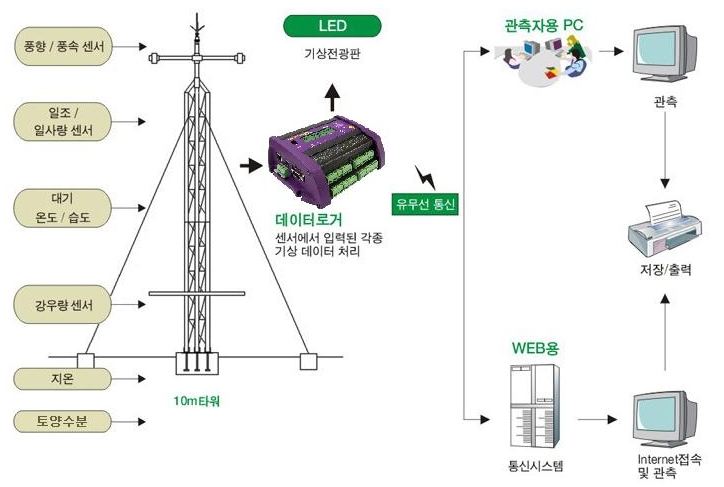
\includegraphics{aws.png}

기본적으로 네트워크에 연결되어 있을 수 밖에 없는 기지국, 라우터와 같은 통신 장비들은 snmp 프로토콜을 이용하여 초창기부터 원격관리가 가능하였다. snmp의 탄생적 특성상 주로 데이터의 입출력량을 모니터링할 수 있으며, UPS등의 전력시스템을 위한 전력 관련 정보들도 수집할 수 있다. NMS (Network Management System)는 snmp를 기본으로 통신장비들의 상황을 모니터링하고 제어할 수 있는 네트워크 통합 관리 시스템이다. 최근에 클라우드 서비스가 각광 받으면서 이 분야의 중요성도 부각되고 있다.

공장 자동화 분야에서도 본 글에서 논하고자하는 원격 시스템 모니터링이 사용된다. SCADA 시스템이라고 많이 불리는 이 시스템에서는 modbus, profibus 등의 단순한 프로토콜을 이용한다. 이 프로토콜들은 주로 근거리 통신을 위한 규격이지만,
원격으로 데이터를 전송할 때는 TCP/IP 상에 데이터를 실어 보내는 방법들을 제공한다.

이상에서 우리가 흔히 알고 있는 컴퓨터 급의 장비들을 관리하기 위한 snmp와
좀더 단순한 공장 자동화 장비들을 모니터링하고 제어하기 위한 modbus,
profibus 프로토콜들이 사용되고 있는 것을 간단히 설명하였다. 본 글에서는
범용 컴퓨터 급이 아닌 센서 등의 단순한 컴퓨터들에서 수집되는 정보들을
어떻게 서버로 전달하고 이렇게 서버에 모아진 정보들을 운영자에게 보여줄
것인지를 설명하고자 한다. 특히 최근에 화두가 되고 있는 big data, Internet
of Things, M2M 등에서도 이러한 내용들이 유용하게 활용될 수 있을 것으로
생각한다.
또한 본 글에서는 ubuntu 리눅스를 기반으로 한 소프트웨어적인 측면만을 다룬다.


\chapter{원격 시스템 모니터링}
\label{monitoring::doc}\label{monitoring:id1}
이 글에서 언급하고자 하는 원격 시스템이란 유선통신 연결이 매우 어려운 지역에서 상용이동통신망을 이용하여 서버와 통신하는 장비를 의미한다. 원격시스템은 스스로 센서를 가지고 있을 수도 있으며, 근거리에서 시리얼 통신을 이용하여 데이터를 수집할 수 있다. 이렇게 수집한 데이터를 서버로 전송하고 서버에서 들어오는 제어신호를 처리할 수 있다. 원격 시스템은 ubuntu 리눅스를 OS로 사용하는 것을 가정한다.


\section{원격 시스템 접근}
\label{monitoring:id2}
원격 시스템들은 원격지에 분산되어 있기 때문에 시리얼 콘솔을 이용해서 장비에 접근하는 것이 번거롭고 시간을 많이 소비하게 된다. 때문에 원격에서 시스템에 접근할 수 있는 방법을 제공하여야만 하며 이 경우, 디버깅과 업데이트가 용이해진다.

하지만, 원격 시스템은 상용이동통신망을 이용하기 때문에 외부에서 직접 접근이 불가능하다. 이런 경우에 접근을 할 수 있는 방법으로 reverse ssh tunnel 이 있다. 먼저 원격 시스템에서 서버로 “ssh -R” 옵션을 사용하여 역방향 터널을 만든다. 이렇게 하면, 원격시스템의 특정 포트에서 ssh 접속을 대기하도록 설정한다.

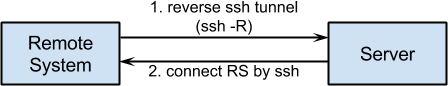
\includegraphics{ssh.png}


\subsection{reverse ssh 터널 생성}
\label{monitoring:reverse-ssh}
ssh 는 보통 ssh 서버에 접속해 원격에서 서버를 관리할 목적으로 많이
사용된다. 클라이언트와 서버 사이에 교환되는 패킷들을 암호화하기 때문에
telnet보다 훨씬 안전하여 많이 사용되는 명령어이다. 하지만, ssh는
telnet 처럼 단순한 기능만을 제공하는 것은 아니다.
본 절에서는 ssh -R 옵션을 통해 reverse 터널을 열어 사용하는 방법을
기술하고자 한다.

두 host A와 B가 있을때 A는 공인IP를 가지고 있지만, B는
사설IP만을 가지고 있다고 할 경우, 일반적으로 B에서 A로만 접근이 가능하다.
하지만, Reverse tunnel을 생성할 경우 A에서 B로의 접근이 가능해 진다.
예를 들어 설명하면, 여러분 가정에 사설IP만을 가지고 있는 리눅스 장비가
있을 경우, 외부에서 집에 있는 리눅스로 접속하여 관리를 할 수 있다.

-R 옵션의 명령어 형태는 아래와 같다. 이 명령은 아래 그림의 client에서 수행하는 것이다.

ssh 터널은 다양한 용도로 사용된다.
위의 그림에서
ssh -fN -R 40122:localhost:22 root@emon-it.net


\subsection{자동 ssh 로그인}
\label{monitoring:ssh}
host A에서 host B의 user b로 로그인하는 것을 가정하고 아래와 같은 명령을 수행하면 A에서 B로 ssh 접속을 할 때 비밀번호를 입력하지 않아도 된다.
아래는 모두 host A에서 수행할 일들이다.
\begin{enumerate}
\item {} 
인증키 생성

\end{enumerate}

\begin{Verbatim}[commandchars=\\\{\}]
\$ ssh-keygen -t rsa
  -t : 생성할 Key의 type (rsa1, dsa, ecdsa, rsa(for protocol 2))
  물어보는 내용에 대해 전부 엔터만 입력하면 된다.
\end{Verbatim}
\begin{enumerate}
\setcounter{enumi}{1}
\item {} 
host B에 .ssh 폴더 생성

\end{enumerate}

\begin{Verbatim}[commandchars=\\\{\}]
\$ ssh user\_b@host\_B mkdir -p .ssh
\end{Verbatim}
\begin{enumerate}
\setcounter{enumi}{2}
\item {} 
인증키 복사

\end{enumerate}

\begin{Verbatim}[commandchars=\\\{\}]
\$ cat .ssh/id\_rsa.pub \textbar{} ssh user\_b@host\_B 'cat \textgreater{}\textgreater{} .ssh/authorized\_keys'
\end{Verbatim}

\begin{notice}{note}{Note:}
2, 3의 과정을 한번에 수행하기

\$ ssh-copy-id \href{mailto:user\_b@host\_B}{user\_b@host\_B}
\end{notice}

\begin{notice}{note}{Note:}
루트권한으로 수행하는 프로세스내에서 원격지로 ssh 접속을 시도할 경우는
루트 계정에서 위의 작업들을 수행해 주어야 한다. 즉 host A에서 어느 계정으로
위의 과정을 수행하는가도 중요하다. 루트 계정에서 자동 로그인을 하기 위해서는
아래 명령어를 먼저 수행한 후 위 과정을 실행하라.

\$ sudo su -
\end{notice}
\begin{description}
\item[{ssh 터널을 만드는 방법은 아래 사이트들을 참고하라.}] \leavevmode\begin{itemize}
\item {} 
\href{http://ymkimit.blogspot.com.au/2013/04/ssh-r-reverse-tunnel.html}{http://ymkimit.blogspot.com.au/2013/04/ssh-r-reverse-tunnel.html}

\item {} 
\href{http://www.hanb.co.kr/network/view.html?bi\_id=547}{http://www.hanb.co.kr/network/view.html?bi\_id=547}

\item {} 
\href{http://blog.kxr.me/2013/02/reverse-ssh-tunnel-manager-remote-ssh.html}{http://blog.kxr.me/2013/02/reverse-ssh-tunnel-manager-remote-ssh.html}

\end{itemize}

\end{description}

ssh -R 옵션
reverse ssh tunneling

주기적인 접근 : 역방향 대기?



\renewcommand{\indexname}{Index}
\printindex
\end{document}
